
\section{Experimental Evaluation}

\subsection{Experimental Setup}

% \begin{table*}
%  \caption{Benchmarks Characteristics %\cite{bienia08characterizationreport}\cite{woo1995splash}\cite{southern2016analysis}}
%  \center
%  \label{BC}
%   \scalebox{1}{
%   \begin{tabular}{ p{3cm} | p{3cm} | p{3cm} | p{3cm} | p{3cm} }
%     \toprule[1pt]
%     Name & Type of Parallelism & Synchronization Rate & Comm/Comp Ratio & Number Threads \footnote{$n$ is the input parameter.} \\
%     \toprule[1pt]
 %   blackscholes & data-parallel & low & high & 1 + n \\
  %  bodytrack & data-parallel & medium & high & 2 + n\\
  %  dedup & pipline & medium & high & 3 + 3n\\
  %  ferret & pipline & high & medium & 3 + 4n\\
  %  fluidanimate & data-parallel & very high & low & 1 + n\\
  %  freqmine & data-parallel & high & high & n\\
  %  swaptions & data-parallel & low & low & 1 + n\\
  %  radix & data-parallel & low & high & n\\
  %  lu\_ncb & data-parallel& low & low & n \\
  %  lu\_cb & data-parallel& low & low & n\\
  %  ocean\_cp & data-parallel & low & low & n\\
  %  water\_nsquared & data-parallel& medium & medium & n\\
  %  water\_spatial & data-parallel& low & low & n\\
  %  fmm & data-parallel& medium & low & n\\
  %  fft & data-parallel& low & high & n\\
   %   \midrule
%     \bottomrule
%  \end{tabular}}
%\end{table*}

 \begin{table}[htbp]
  \caption{Benchmarks Characteristics \cite{bienia08characterization}\cite{woo1995splash}\cite{southern2016analysis}}
  \center
  \label{BC}
   \scalebox{1}{
   \begin{tabular}{ p{2.3cm} |  p{1.8cm} | p{1.8cm} | p{1.4cm} }
     \hline
     Name & Sync. Rate & Comm/Comp Ratio & No. Threads\\
    \hline
    blackscholes &  low & high & 1 + n \\
    bodytrack &  medium & high & 2 + n\\
    dedup &  medium & high & 3 + 3n\\
    ferret &  high & medium & 3 + 4n\\
    fluidanimate &  very high & low & 1 + n\\
    freqmine &  high & high & n\\
    swaptions &  low & low & 1 + n\\
    radix &  low & high & n\\
    lu\_ncb & low & low & n \\
    lu\_cb &  low & low & n\\
    ocean\_cp &  low & low & n\\
    water\_nsquared &  medium & medium & n\\
    water\_spatial &  low & low & n\\
    fmm &  medium & low & n\\
    fft &  low & high & n\\
    \hline
    % \bottomrule
  \end{tabular}}
\end{table}

\textbf{\textit{Experimental Environment:}} We ran our experiments on GEM5, simulating an ARM big.LITTLE-like architecture. The big cores are similar to out-of-order 2 GHz CortexA57 cores, with a 49 KB L1 instruction cache, a 32 KB L1 data cache, and a 2 MB L2 cache. The little cores are similar to in-order 1.2 GHz CortexA53 ones, with a 32 KB L1 instruction cache, a 32 KB L1 data cache, and a 0.5 MB L2 cache. We evaluated three distinct hardware configurations, including two symmetric configurations - one with two big and two little cores (2B2S) and one with four big and four little ones (4B4S), and two asymmetric configurations - one with two big and four little cores (2B4S) and one with four big cores and two little cores (4B2S). The OS is Linux v3.16. We cross-compiled the kernel with gcc v5.4.0, while we compiled the benchmarks inside the emulated environment with gcc v4.8.2.

 \begin{table*}
  \caption{Multi-programmed Workloads Compositions}
  \center
  \label{WC}
   \scalebox{1}{
   \begin{tabular}{ p{2cm} | p{7cm} | p{4cm} | p{2cm} }
    \hline
     \multicolumn{4}{c}{Synchronization-intensive VS Non-synchronization-intensive Workloads}\\
    \hline
     Index & Workload Composition & Synchronizations & Threads \\
    \hline
    Sync - 1 & water\_nsquared - fmm & intensive & 4 \\
    Sync - 2 & dedup - fluidanimate & intensive & 18 \\
    Sync - 3 & water\_nsquared - fmm - fluidanimate - bodytrack & intensive & 9 \\
    Sync - 4 & dedup - ferret - fmm - water\_nsquared & intensive & 20\\
    \hline
    NSync - 1 & water\_spatial - lu\_cb & non-intensive & 4 \\
    NSync - 2 & blackscholes - swaptions & non-intensive & 16 \\
    NSync - 3 & radix - fft - water\_spatial - lu\_cb & non-intensive & 8\\
    NSync - 4 & blackscholes - ocean\_cp - lu\_ncb - swaptions & non-intensive & 20\\
     \hline
     \multicolumn{4}{c}{Communication-intensive VS Computation-intensive Workloads}\\
     \hline
     Index & Workload Composition & Comm/Comp & Threads \\
    \hline
    Comm - 1 & water\_nsquared - blackscholes & Communication-intensive & 4 \\
    Comm - 2 & ferret - dedup &  Communication-intensive & 16 \\
    Comm - 3 & water\_nsquared - fft - radix - bodytrack &  Communication-intensive & 9 \\
    Comm - 4 & blackscholes - dedup - ferret - water\_nsquared &  Communication-intensive & 20\\
    \hline
    Comp - 1 & water\_spatial - fmm & Computation-intensive & 4 \\
    Comp - 2 & fluidanimate - swaptions & Computation-intensive & 17 \\
    Comp - 3 & lu\_ncb - fmm - water\_spatial - lu\_cb & Computation-intensive & 8\\
    Comp - 4 & fluidanimate - ocean\_cp - lu\_ncb - swaptions & Computation-intensive & 20\\
    \hline
  \end{tabular}}
  \scalebox{0.9}{
  \begin{tabular}{p{1.5cm} |p{4cm} |p{1cm}|| p{1.5cm} |p{7cm} |p{1cm}}
   \hline 
     \multicolumn{6}{c}{Random-mixed Multi-programmed Workloads}\\
  \hline
      Index & Workload Composition & Threads & Index & Workload Composition & Threads\\
   \hline
    Rand - 1 &lu\_cb - dedup & 19& Rand - 6 &water\_spatial - fmm - fft - fluidanimate &21\\
    Rand - 2 &lu\_ncb - bodytrack &10& Rand - 7 &fmm - water\_spatial - ferret - swaptions&20\\
    Rand - 3 &ferret - water\_spatial&9 & Rand - 8 &water\_spatial - water\_nsquared - ferret - freqmine&17\\
    Rand - 4 &ocean\_cp - fft&8 & Rand - 9 &blackscholes - bodytrack - dedup - fluidanimate&55\\
    Rand - 5 &freqmine - water\_nsquared&6 & Rand - 10 &lu\_cb - lu\_ncb - bodytrack - dedup&53\\
   \hline
  \end{tabular}}
\end{table*}

\textbf{\textit{Workloads:}} For our workloads we used 15 different benchmarks. They are pulled either from PARSEC3.0~\cite{bienia11benchmarking} ({\it blackscholes, bodytrack, dedup, swaptions, freqmine, ferret and fluidanmiate}) or from SPLASH2~\cite{woo1995splash} ({\it radix, lu\_ncb, lu\_cb, ocean\_cp, water\_nsquared, water\_spatial, fmm and fft}). 
\footnote{It is a common issue that the applied version of GEM5 simulator does not fully support all PARSEC3.0 benchmarks on ARM and previous gem5-based research use a selection of PARSEC3.0 benchmarks for evaluation~\cite{endo2014micro,gallego2016dram,van2013full} and IO-redirection issues prevent us applying more SPLASH2 benchmarks with additional input files to keep same order of magnitude in our ARM disk image for simulation.}
%We added another two single-threaded benchmarks ({\it mcf, bzip2}) from SPEC CPU2006~\cite{henning2006spec} to complicate scheduling decisions. 
All benchmarks use pthread-based parallelism apart from \emph{freqmine} which does not support pthreads, only OpenMP. To keep the simulation time reasonably short, we use the \emph{simsmall} inputs for the multi-threaded benchmarks.
%For \emph{mcf} we use the reference input, while for \textit{bzip2} we used the source reference input. We edited the source files of \textit{mcf} and \textit{bzip2} to limit the number of iterations of their outermost loops to 3000 for the former and 250 for the latter, to keep their runtimes in the same order of magnitude as the multi-threaded benchmarks.
%It is a common issue that GEM5 simulator does not support all PARSEC3.0 benchmarks well \cite{endo2014micro}, so we also applied several more SPLASH2 benchmarks \cite{woo1995splash}: {\it radix, lu\_ncb, lu\_cb, ocean\_cp and fft}. We also considered two more single-thread benchmarks ({\it mcf, bzip2}) from SPEC2006 \cite{henning2006spec} to make the tested multiprogrammed workloads further complicated. 

The benchmarks characteristics are shown in Table~\ref{BC}. Where $n$ in the number of threads denotes the input parameter of the PARSEC3.0 benchmarks~\cite{southern2016analysis}. Runtime synchronizations of PARSEC3.0 and SPLASH2 bechnmarks are cased by barriers, locks, conditions and pauses~\cite{bienia2008parsec,woo1995splash}. We group the benchmarks into two classes for structural comparison:
\begin{itemize}
    \item Synchronization intensive or not.
    \item Communication or computation intensive.
\end{itemize}

For each classes, we further generate workloads to be different on both number of applications and number of total threads. Beyond that, we also randomly mix our selected benchmarks to build additional multi-threaded multi-programmed workloads with random number of total application threads.
%We randomly mix our selected benchmarks to build workloads with either multiple multi-threaded applications or mixed multiple multi-threaded and single-thread applications. 
Table~\ref{WC} shows the workloads we used. For all workloads, we boot the simulated system, start the benchmarks, and wait until they reach the end of their initialization. This is done with fast simulation. When all benchmarks are initialized, we switch to cycle accurate simulation and resume the execution of the benchmarks. We only collect statistics for the cycle accurate part of the simulation.

Each one of our results represents the average over two simulations with different core orders - either big cores first or little cores first. The initial state of the system can have a significant impact on performance. For the Linux scheduler in particular, the order of starting benchmarks will decide which benchmarks will be initially assigned to big and little cores. By randomizing the initial state and especially the execution order of the workload benchmarks for each simulation, we minimize the effect of randomness on our evaluation.

%The number of parallel threads for benchmarks from SPLASH2 can be setup easily as in input arguments, while for PARSEC benchmarks, we only setup the lower bound of threads and the program will then determines the actual number of threads based on the relationships described in \cite{southern2016analysis}. To avoid dominating system performance by a single benchmark in each workload, we normalized the number of threads from different benchmarks to be similar and keep the input sizes of all applications to be {\it simsmall}. 
%The only exception is on benchmark {\it streamcluster} from PARSEC3.0 - it is a known issue \cite{southern2016analysis,roth2012deconstructing} that increasing the number of threads to be greater than 4 will significantly decrease the performance of this benchmark because of its barrier based synchronization.

\textbf{\textit{Metrics:}} Our evaluation uses two metrics to quantify scheduling efficiency: {\it Heterogeneous Average Normalized Turnaround Time} (H\_ANTT) and {\it Heterogeneous System Throughput} (H\_STP). They are based on ANTT and STP, as introduced in~\cite{eyerman2008system}. For an application mix, both ANTT and STP use the runtime of each application when executed on its own, i.e. when there is no resource sharing and scheduling decisions have little effect. ANTT expresses the average slowdown of all applications in the mix, with the slowdown for each application being relative to its isolated runtime. STP expresses the sum of the relative throughputs for all applications, again relative to the isolated throughput.

For AMPs, these two metrics fail to work as intended. The runtime when executed alone is still affected by scheduling decisions, e.g. which threads to run on big cores. To overcome the problem, our modified metrics H\_ANTT and H\_STP use the runtime of each application in the mix when executed alone \emph{on a system where there are only big cores}. If the turnaround time of each application $i$ while being co-scheduled is $T^{M}_i$ and the turnaround time for the same application when running alone on a big-only system is $T^{SB}_i$, then:

$$ H\_ANTT = \frac{1}{n}\sum^{n}_{i=1}\frac{T^{M}_i}{T^{SB}_i}$$
$$ H\_STP = \sum^{n}_{i=1}\frac{T^{SB}_i}{T^{M}_i}$$

When we evaluate a single benchmark on its own, we use the {\it Heterogeneous Normalized Turnaround Time} (H\_NTT):

$$ H\_NTT = \frac{T^{M}}{T^{SB}}$$

H\_ANTT and H\_NTT are better when lower, H\_STP is better when higher. For most figures, we further normalize our results relative to the Linux CFS results for the same configuration and workload.

\textbf{\textit{Schedulers:}}
We compare COLAB against the Linux CFS scheduler~\cite{molnar2007cfs} and a scheduler based on WASH~\cite{jibaja2016portable}. WASH is implemented inside a Java VM and is meant to control the affinities of Java threads only. Our implementation uses the same heuristic as the original WASH but is part of the Linux scheduler and controls all application threads. Additionally, we replaced the WASH core sensitivity model with one built from scratch for our hardware configuration and our set of performance counters, using the same process as described in the WASH paper.

\begin{figure}
\centering
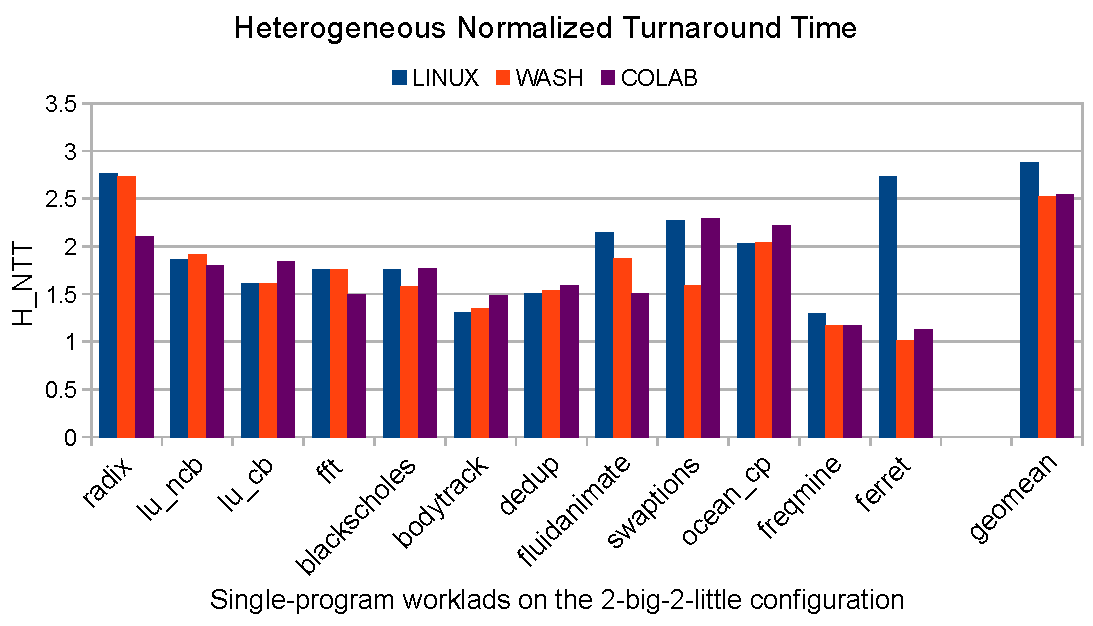
\includegraphics[scale=0.45]{figures/MSW2.pdf}
\caption{Heterogeneous Normalized Turnaround Time (H\_NTT) of single program workloads.  All results are normalized to the Linux CFS ones. Lower is better}
\label{MSW}
\end{figure}  

%\begin{figure*}
%\centering
%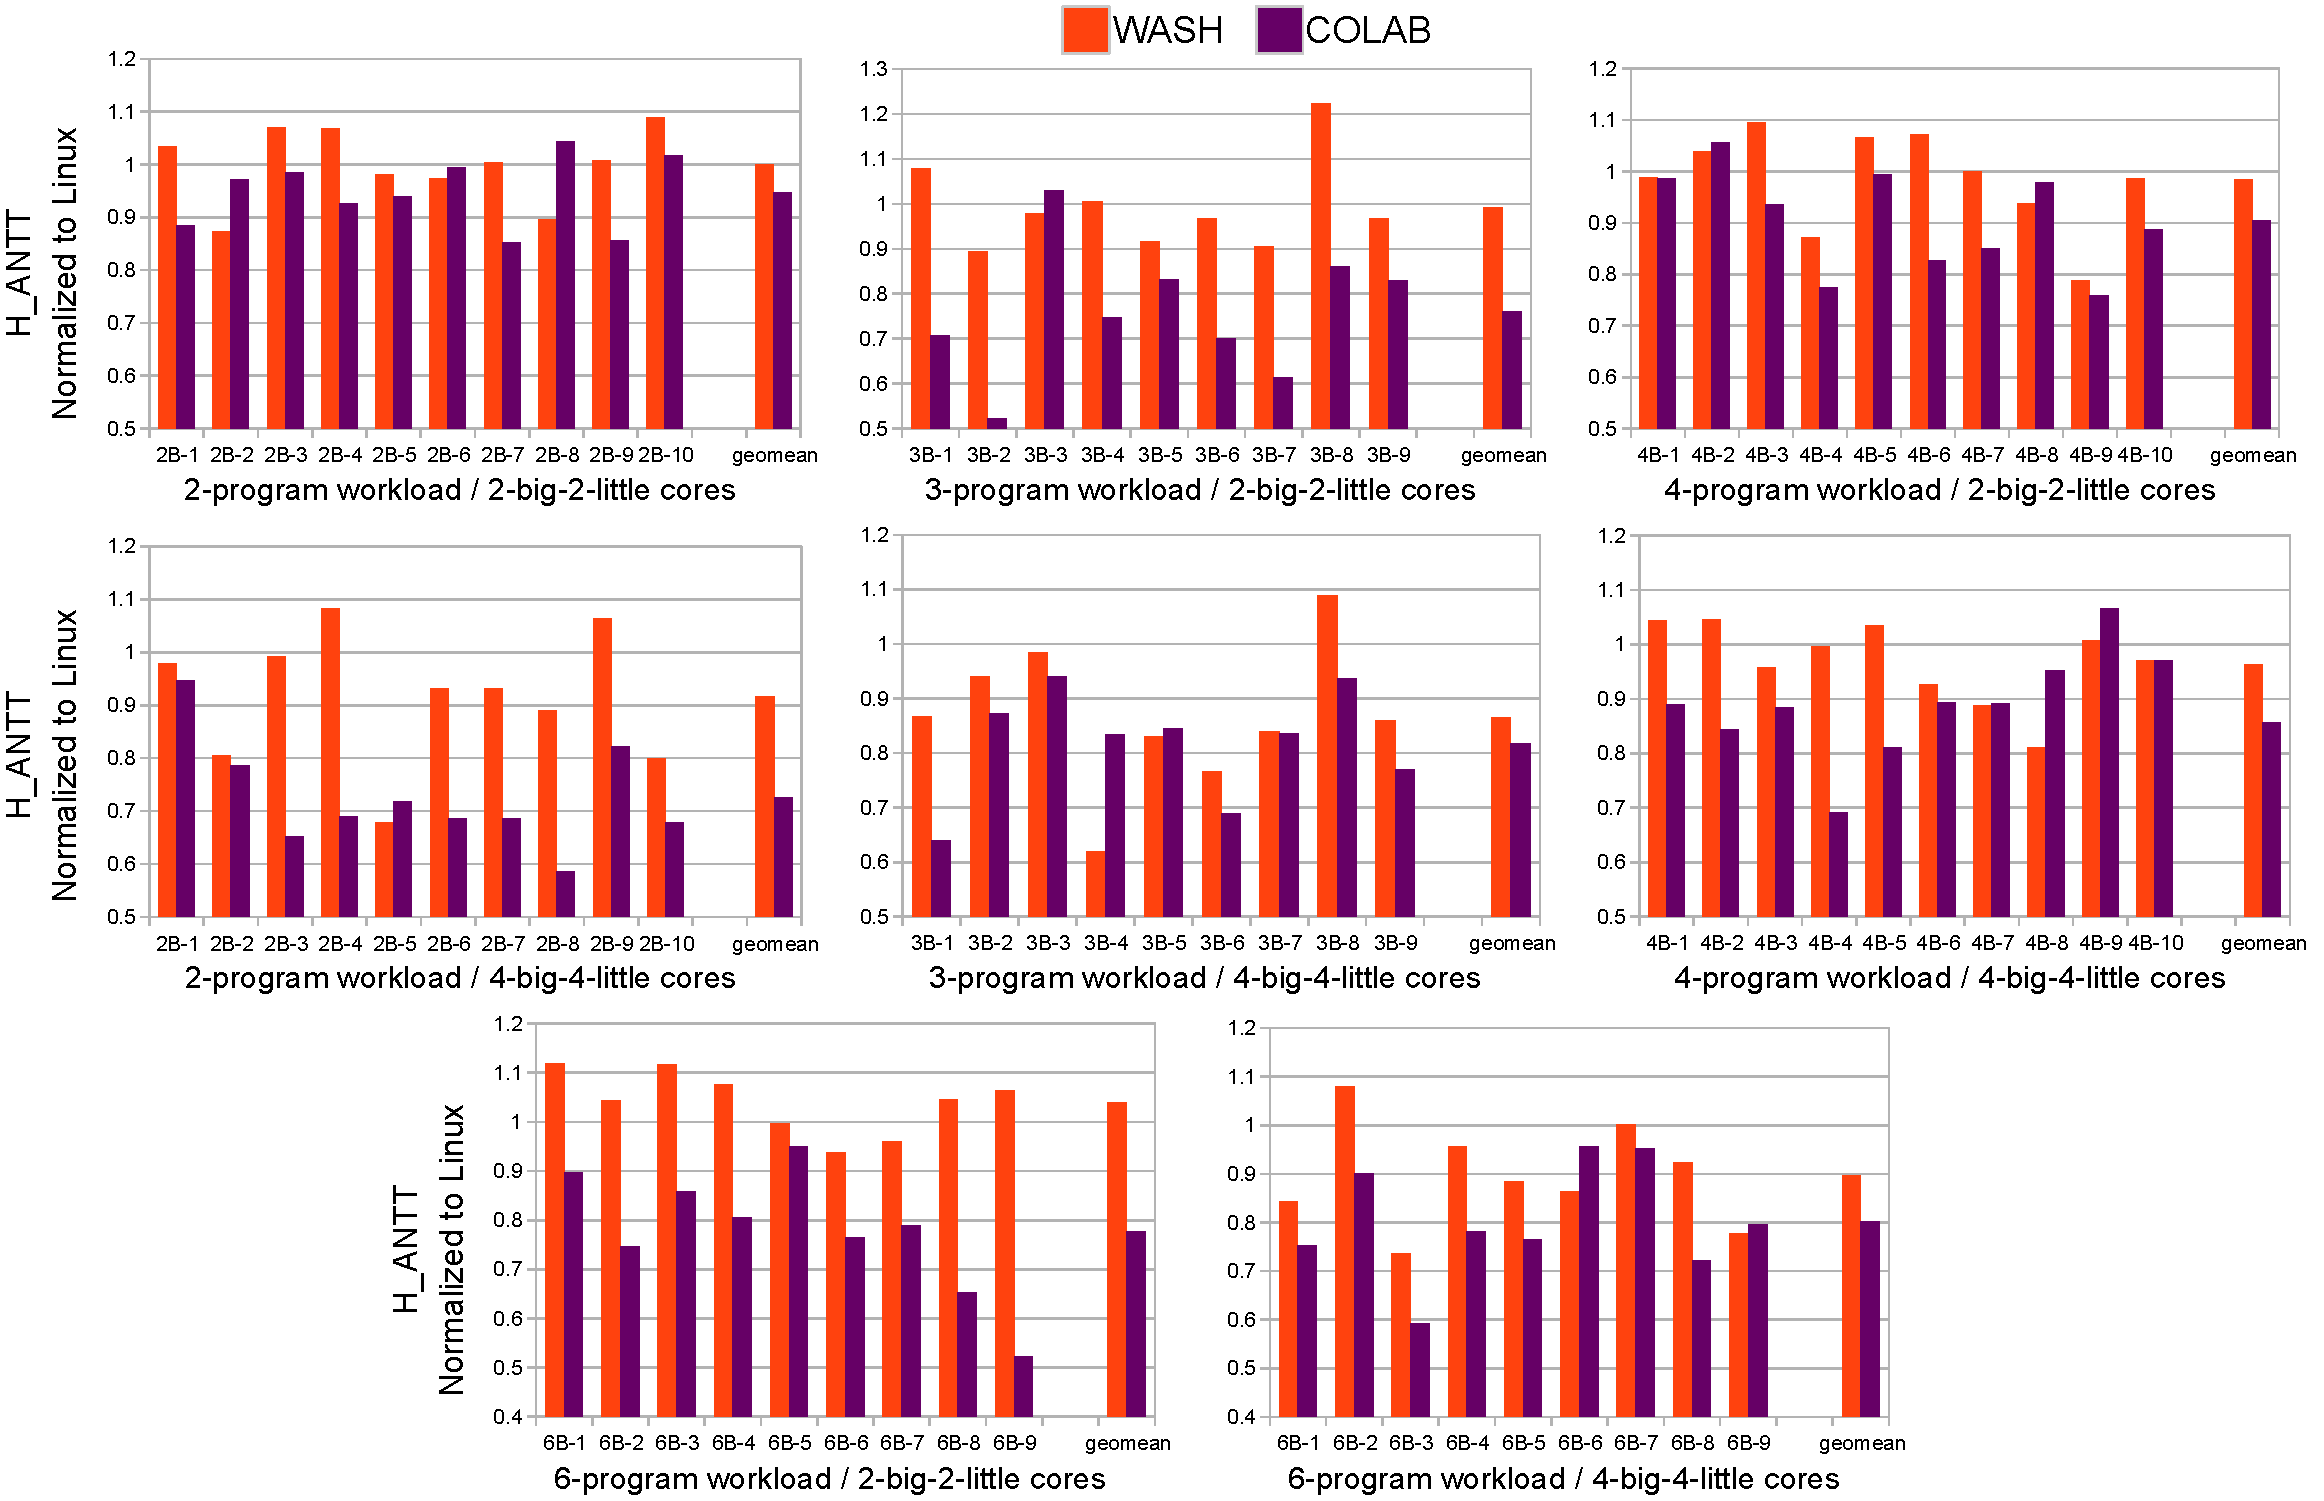
\includegraphics[scale=0.4]{figures/HANTT_NEW.pdf}
%\caption{Heterogeneous Average Normalized Turnaround Time (H\_ANTT) of multiprogrammed workloads on 2-big-2-little and 4-big-4-little configurations. All results are normalized to the Linux CFS ones. Lower is better.}
%\label{M24W}
%\end{figure*}


\subsection{Experimental Results and Analysis}

\subsubsection{Single-programmed Workloads}
Much of the research on AMP scheduling focuses on single-programmed workloads. In this context, fairness and load balancing are not important, the focus is on core sensitivity and bottleneck acceleration. In this section, we examine how COLAB fares under this scenario. Figure~\ref{MSW} shows Heterogeneous Normalized Turnaround Time for our multi-threaded benchmarks when executed alone on a 2-big-2-little hardware configuration. For each configuration and benchmark we present three bars, Linux(blue), WASH(red) and COLAB(violet). 
Three SPLASH2 benchmarks $fmm$, $water\_nsquared$ and $water\_spatial$ do not support more than 2 threads with $simsmall$ input size on GEM5, so we do not present those 2-threaded benchmarks: scheduling them optimally for performance is trivial.

The AMP-agnostic Linux scheduler is inappropriate for most benchmarks. COLAB improves H\_NTT by up to 58\% and by 12\% on average. Our best result relative to Linux is for \emph{ferret}. Most computation happens in a pipeline pattern but its stages are not balanced. AMP-aware schedulers take advantage of that by scheduling the longest stages, the bottleneck threads, on big cores. As a result, COLAB does only 13\% worse than running on a system \emph{with four big cores}, while CFS executes the benchmark 173\% slower.

Our best result relative to WASH is for \emph{fluidanimate}. Previous work~\cite{bienia08characterization} has shown that \emph{fluidanimate} has around 100x more lock-based synchronizations than other PARSEC benchmarks. Our collaborative core allocation and thread selection policy is much better than WASH at prioritizing bottleneck threads.  As a result, we reduce turnaround time by 30\% compared to Linux and 20\% compared to WASH.

In some cases, such as \emph{bodytrack}, \emph{lu\_ncb}, or \emph{freqmine}, AMP-awareness has little effect on performance. Such benchmarks split work dynamically between threads, so they adapt to asymmetries in processing speed. Moreover, all threads executed the same code and display similar core sensitivity, so there is no benefit in assigning specific threads to specific cores. When either WASH or COLAB interfere with scheduling decisions, they are more likely to make wrong decisions or introduce overhead than help. Such behavior was also apparent in the original WASH paper~\cite{jibaja2016portable}. The pipeline benchmark \emph{dedup} has five stages to stream the input set. When the number of threads is greater than the number of cores that can be run, both heterogeneous-aware schedulers can not service the excess threads in time, resulting in a certain impact on overall system performance.

There is only one case where COLAB performs significantly worse than WASH. For \emph{swaptions}, we perform as well as the AMP-agnostic Linux scheduler while WASH improves turnaround time by 31\%. This is because the bottleneck threads of \emph{swaptions} are core insensitive while the non-bottleneck threads are core sensitive. This being the ideal case for WASH, it improves turnaround time while we fail to do the same.

On average, WASH and COLAB perform similarly well and improve performance by 12\% compared to Linux when handling single program workloads. This is a limited scenario, with no need for fairness and a simple decision space. COLAB was not expected to perform much better than the state-of-the-art, doing as well as it is a positive result.


\subsubsection{Multi-programmed Workloads}
The main aim of the COLAB scheduler is to target workloads of multiple multi-threaded programs, which represents the most general case for CPU scheduling. In this section, we evaluate the performance of COLAB in this setting, under four different hardware configurations (2B2S, 2B4S, 4B2S, 4B4S), comparing it with both Linux and WASH scheduler on 26 different workloads listed in Table~\ref{WC}. The workloads are composed to represent different configuration of applications based on their rate of synchronisation, communication-to-computation ratio and the number of application threads. Based on this, we classify workloads into different sets:

\begin{itemize}
\item \textbf{Synchronisation-intensive} workloads comprise of the programs that have high synchronisation rate. Our hypothesis was that these workloads contain more bottleneck threads, due to intensive synchronisation between different threads, and that the mechanisms we developed in COLAB scheduler will schedule these threads in more optimal way, compared to Linux and WASH schedulers. On the other hand, \textbf{Synchronisation-Nonintensive} workloads comprise of the programs that have low synchronisation rate, hence giving less opportunities to the COLAB scheduler to improve on Linux and WASH schedulers. Therefore, for these workloads we expected to see less impact from COLAB.
\item \textbf{Communication-intensive} workload comprise of the programs that have high communication-to-computation ratio. This result in high volume of communication between program threads, which furher results not only in more bottleneck threads, but also in low amount of computation done by some threads. This scenario gives more opportunities to COLAB for improved scheduling decisions, therefore our hypothesis was that for these workloads we will get better results than Linux and WASH. \textbf{Computation-intensive} workloads comprise of applications that have high computation-to-communication ratio. Due to less bottleneck threads and more similarity in terms of computation load of each thread, there are less opportunities for the COLAB scheduler here to improve on Linux and WASH, therefore we expected similar results between all three scheduler.
\item \textbf{Mixed} workloads represent the most general workloads, comprising a mixture of synchronisation-intensive, synchronisation-nonintensive, communication-intensive and computation-intensive programs. The intention of using these workload is to observe how well COLAB performs in general setting, compared to Linux and WASH.
\end{itemize}

\begin{figure}
\centering
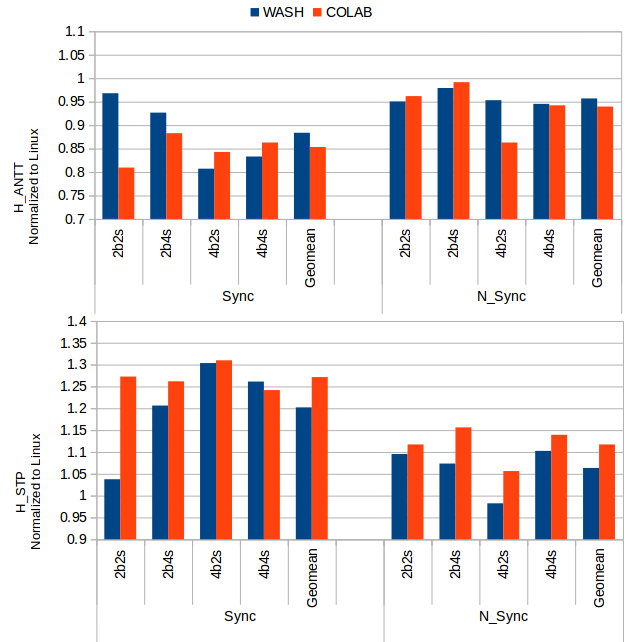
\includegraphics[scale=0.39]{figures/sync.png}
\caption{Heterogeneous Average Normalized Turnaround Time (H\_ANTT) and Heterogeneous System Throughput (H\_STP) of Synchronization-Intensive and Non-Synchronization-Intensive Workloads. All results are normalized to the Linux CFS ones. Lower is better for H\_ANTT and higher is better for H\_STP.}
\label{sync}
\end{figure} 

\paragraph{Synchronisation Intensive vs. Synchronisation Nonintensive Workloads} Figure~\ref{sync} shows the performances of all three scheduler on synchronization-intensive (\emph{Sync}) and synchronization-nonintensive \emph{N\_Sync} workloads. As with the other experiments in this section, the experiments here are grouped based on hardware configuration on which they are exceuted. We present the mean H\_ANTT and H\_STP over four different workloads (see Figure~\ref{fig:XX}). Note again that lower H\_ANTT and higher H\_STP translate into higher performance of the scheduler. We can observe that, for synchronisation-intensive workloads, COLAB improves turnaround time by around 15\% and 4\% on average compared to Linux and WASH, respectivelly. We can also observe that on the hardware configurations with smaller number of cores (2B2S), the COLAB scheduler performs especially well compared to Linux and WASH, improving over Linyx by up to 20\% and over WASH by up to 16\%. This is because Linux and WASH show their limitations in a scenario where limited amount of resources is available and where there are multiple bottleneck threads coming from different programs. WASH places all bottleneck threads onto the big cores, which results in these threads having to wait for CPU time in busy run queues, ending up with only 3\% of performance improvement over Linux. The COLAB scheduler handles these bottleneck threads in a more holistic way, improving performance by 20\% and system throughput by 27\%, compared to Linux.

%Synchronization-intensive workloads fully composed by benchmarks with higher synchronization rates than others, which lead to the  much more importance of multiple bottlenecks and critical threads co-acceleration. Both heterogeneous-aware schedulers can show a significant advantage than Linux CFS on these cases. As a result, COLAB improves turnaround time by around 15\% compared to Linux and around 4\% compared to WASH on average of different configurations and workload compositions. On certain workloads and configuration cases, COLAB can outperform Linux by up to 20\% (2B2S) and outperform WASH by up to 16\% (2B2S). 
%The state-of-the-art WASH scheduler shows its limitations when used on limited resources (2B2S). With increasing  pressure  from  co-executed  applications, properly  balancing  bottleneck  acceleration and core sensitivity across multiple programs using only two big cores becomes difficult. WASH identifies these bottlenecks and assigns their threads to big cores without further consideration. Instead of accelerating the bottleneck threads, this leads to the bottleneck threads getting stuck waiting for CPU time in busy runqueues. At the same time, non-critical threads enjoy short waiting times on little cores. WASH ends up performing only 3\% better than Linux CFS. COLAB handles bottleneck threads in a more holistic way, improving performance around 19\% for the same scenario.
%Similar results are presented for the system throughput. COLAB outperform Linux by around 27\% and outperform WASH by around 7\%. 

As for synchronization-nonintensive workloads, neither COLAB nor WASH have a significant optimization space, since there are not enough bottleneck and critical threads that can be accelerated. As a result, both schedulers perform similarly to Linux, with COLAB improving turnaround time and system throughput by around 6\% and 12\% compared to Linux and around 2\% and 5\% compared to WASH. \textbf{VJ: 12\% seems quite significant, though.} \textit{This verifies our hypothesis that heterogeneity-aware schedulers bring more benefit, compared to the Linux scheduler, for workloads that are dominated by synchronisation-intensive programs. Furthermore, the COLAB scheduler notably outperforms the state-of-the-art WASH scheduler on limited-resource hardware configurations.}

\begin{figure}
\centering
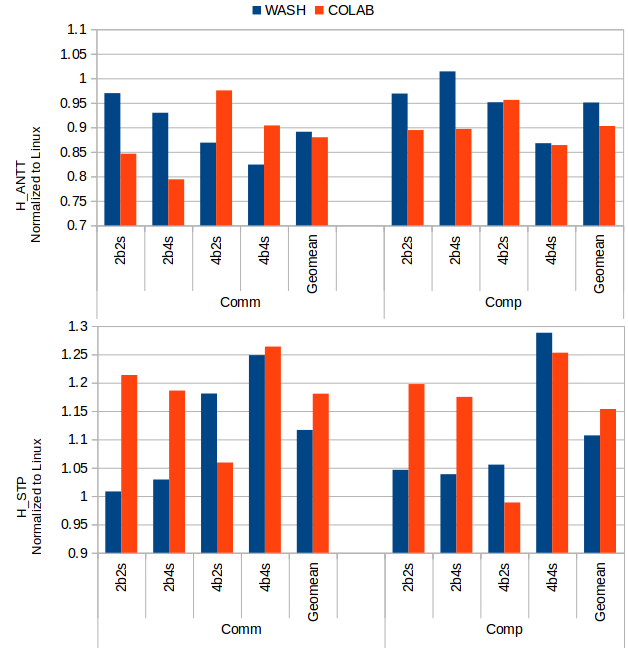
\includegraphics[scale=0.39]{figures/com.png}
\caption{Heterogeneous Average Normalized Turnaround Time (H\_ANTT) and Heterogeneous System Throughput (H\_STP) of Communication-Intensive and Computation-Intensive Workloads. All results are normalized to the Linux CFS ones. Lower is better for H\_ANTT and higher is better for H\_STP.}
\label{com}
\end{figure} 

\begin{figure}
\centering
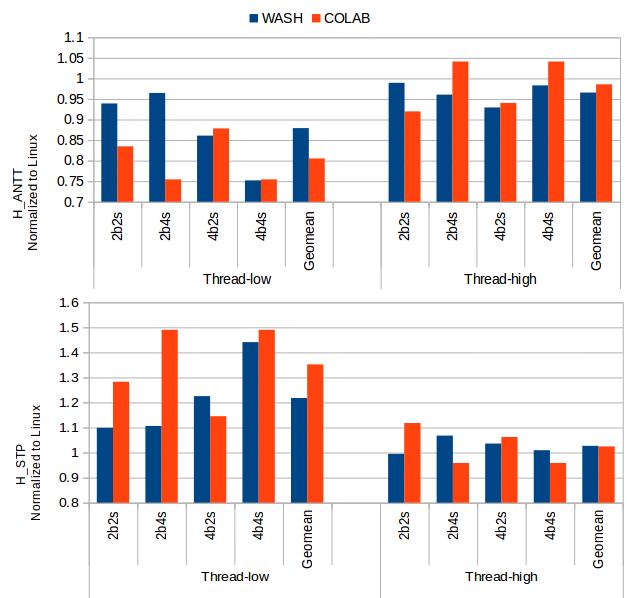
\includegraphics[scale=0.35]{figures/nthread.png}
\caption{Heterogeneous Average Normalized Turnaround Time (H\_ANTT) and Heterogeneous System Throughput (H\_STP) of low number of application threads and high number of application threads Workloads. All results are normalized to the Linux CFS ones. Lower is better for H\_ANTT and higher is better for H\_STP.}
\label{nthread}
\end{figure} 

\paragraph{Comminication-intensive vs. Computation-intensive Workloads} Figure~\ref{com} shows the performance of COLAB, WASH and Linux schedulers on communication-intensive and computation-intensive workloads. 
%The hardware configuration is indicated on the X-axis of each subplot. Lower H\_ANTT and higher H\_STP translates into higher performance.
%Communication intensive workloads fully composed by benchmarks with high communication-to-computation ratio, which lead to a significant amount of intra-program communications between multiple application threads. This can result in not only multiple runtime bottlenecks, but also light computation of each thread. So multiple bottlenecks need to be co-executed and each of them has lighter computation need to be done.
Both COLAB and WASH schedulers improve the Linux scheduler. They, however, offer different advantages on different hardware configurations. COLAB distributes the bottleneck threads to both big and little cores, which results in more significant improvements on limited big-core cases (2B2S, 2B4S). COLAB improves the turnaround time by up to 21\% compared to Linux and 15\% compared to COLAB on the 2B4S configuration. As is the case with the synchronisation-intensive workloads, WASH accumulates the bottleneck threads on big cores only, which results in a better performance where there are enough big-core cases (4B2S, 4B4S). On these configurations, WASH improves turnaround time by up to 18\% over Linux (on 4B4S configuration) and up to 10\% over COLAB (on 4B2S configuration). On average, COLAB improves the turnaround time by around 12\% compared to Linux and 1\% compared to WASH for the communication intensive workloads on all configurations. We observe similar results for system throughput, where COLAB outperforms Linux by around 18\% and outperforms WASH by around 5\%.

As noted before, computation-intensive workloads offer less improvement space for both heterogeneity-aware schedulers over Limux. Still, we can observe better performance for COLAB than for WASH and Linux, with COLAB improving turnaround time and system throughput by around 10\% and 15\%, respectivelly, compared to Linux and 5\% compared to WASH. This is, again, due to a fact that multiple bottlenecks are distributed both to big and little cores, which results in more efficient use of the available hardware resources for the few bottlenecks that are present.

\emph{To summarise, heterogeneous aware schedulers show better performance gain on communication-intensive workloads than on computation-intensive workloads. COLAB outperforms WASH on both workloads on average and shows more significant advantage on computation-intensive workloads. WASH only outperforms COLAB on communication-intensive workloads when there are enough high performance big cores available.}
%up to 36\% (Comm-4 on 2B2S) and outperform WASH by up tp 24\% (Comm-3 on 2B4S) on turnaround time.



\begin{figure}
\centering
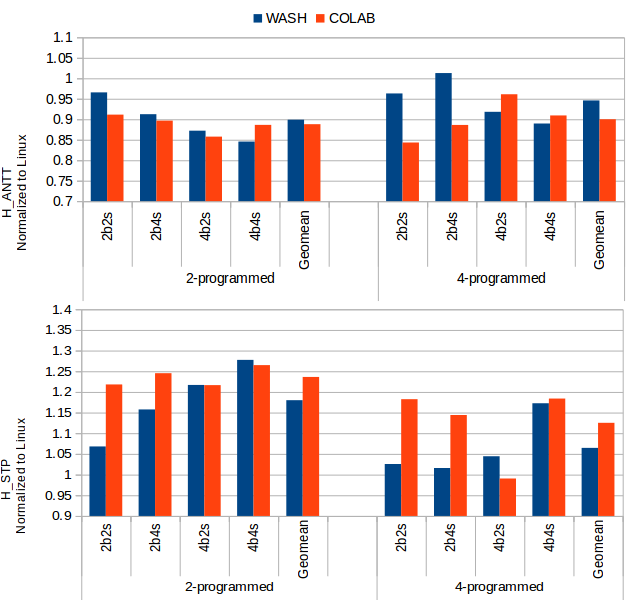
\includegraphics[scale=0.35]{figures/nprog.png}
\caption{Heterogeneous Average Normalized Turnaround Time (H\_ANTT) and Heterogeneous System Throughput (H\_STP) of 2-programmed and 4-programmed Workloads. All results are normalized to the Linux CFS ones. Lower is better for H\_ANTT and higher is better for H\_STP.}
\label{nprog}
\end{figure} 

\begin{figure*}
\centering
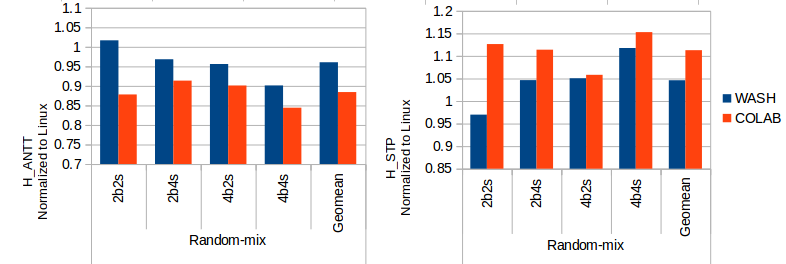
\includegraphics[scale=0.5]{figures/rand.png}
\caption{Heterogeneous Average Normalized Turnaround Time (H\_ANTT) and Heterogeneous System Throughput (H\_STP) of 2-programmed and 4-programmed Workloads. All results are normalized to the Linux CFS ones. Lower is better for H\_ANTT and higher is better for H\_STP.}
\label{rand}
\end{figure*} 

\paragraph{Mixed Workloads}
Figure~\ref{rand} shows the performances of 10 mixed workloads. We can observe that COLAB performs very well for these workloads: more diverse programs mean more asymmetry, more bottlenecks, more type of critical threads and more potential for acceleration. Our collaborative multi-factor scheduler carefully handling all the issues (core sensitivity, thread criticality and fairness) brings a significant performance gain against WASH and Linux on this scenario - COLAB improves turnaround time and system throughput by around 12\% and 11\% compared to Linux and around 8\% and 7\% compared to WASH.

\paragraph{Thread and program count} In our next set of experiments, we studied what impact does the total number of threads and a total number of programs in a workload has on the performance of heterogeneity-aware schedulers. Figure~\ref{nthread} shows the performance of all considered schedulers both for workloads comprising a low number of threads (where there is less threads than cores in the system) and for workloads comprising a high number of threads (where there are significantly more threads than cores). We can observe that both COLAB and WASH perform singificantly better than Linux for workloads with a low number of threads. Fewer threads make it easier to indicate the bottlenecks and critical threads, and then to place them carefully on the appropriate resources - either by migrating them to big cores (WASH and COLAB) or by also giving high priorities to them on little cores (COLAB). With limited big core resources, COLAB does enjoy a more significant performance gain against WASH by distributing those few bottlenecks on both big and little cores to accelerate simultaneously and avoid leaving cores idle. COLAB outperforms Linux by up to 25\% (2B4S) and WASH by up to 21\% (2B4S) on turnaround time. On average, COLAB improves turnaround time and system throughput by around 20\% and 35\% compared to Linux and around 8\% and 11\% compared to WASH for workloads with a low number of threads. For workloads with a high number of threads, neither Linux nor WASH are able to improve much on Linux. Overloading the system with threads means that, regardless of where we place threads, cores will have long run queues. Furthermore, COLAB and WASH do more context switching (due to migration of threads between runqueues), which in this brings significant penalty that cannot be mitigated with good placement of threads. Of the two heterogeneity-aware schedulers, COLAB, with its scale-slice technique, more frequently migrates threads, which results in a slightly worse performance than WASH. On average, COLAB improves turnaround time and system throughput by less than 2\% and 3\% compared to Linux, while WASH slightly outperforms COLAB by 2\% on turnaround time and 0.2\% on system throughput.

\emph{To summarise this set of experiments, heterogeneity-aware schedulers offer significant advantage over Linux on workloads where the number of threads is approximately the same as the number of cores, with COLAB having much better performance than WASH. When the number of threads in workload is significantly higher than the number of available cores, both scheduler perform similarly to Linux with WASH performing slightly better than COLAB.}

%\textbf{\textit{Number of Co-executed Programs:}}
The above results are confirmed when we considered workloads with different number of programs in them. Figure~\ref{nprog} shows the performance of all schedulers for 2-programmed and 4-programmed workloads. We can make similar observations as in the case of workloads with variable number of threads - increasing the number of co-executed programs gives higher pressure on the scheduler, increasing the waiting time of threads in runqueues and reducing the direct benefit of migration between waiting threads.
%. Heterogeneous aware schedulers generally enjoy better performance gain against Linux on workloads with less programs. Similar as the issue in the above comparisons for total number of threads, more programs with more threads increase the waiting list on runqueues and reduce the direct benefit of migrations between waiting programs/threads. While by more intelligent distributed placing critical threads between big and little cores, our COLAB does face less problem than WASH from the pressure of increasing programs. 
As a result, both COLAB and WASH outperform Linux by more than 10\% on 2-programmed workloads on turnaround time and COLAB can keep the 10\% performance gain also on 4-programmed workloads, while WASH reduced to only have 5\% performance gain on 4-programmed workloads. As for system throughput, COLAB improves by 23\% and 12\% on 2-programmed and 4-programmed workloads compared to Linux while improves by 5\% and 6\% on 2-programmed and 4-programmed workloads compared to WASH. \textbf{VJ: This is a bit counterintuitive. Why do we get better results for COLAB scheduler when we have more programs but not when we have more threads in a workload?}


\paragraph{Summary of Experiments} Our experiments showed that the state-of-the-art heterogeneous-aware WASH scheduler struggles to make better scheduling decisions that the Linux schedules for a number of different types of workloads and configurations: synchronization-intensive workloads, computation-intensive workloads, low threads number workloads, high program number workloads, mixed multi-class workloads and limited big cores configurations. Trying to handle both core sensitivity and bottleneck acceleration through thread affinity alone may lead to too many threads assigned to big cores. Instead, we handle the two optimization aims separately. We assign on big cores only threads which run significantly faster on them and we prioritize running bottleneck threads regardless of their thread affinity. This leads to improved turnaround time, higher throughput, and better use of the processor resources compared to both Linux and WASH. In summary from all 312 experiments, COLAB improves turnaround time and system throughput by 11\% and 15\% compared to Linux and by 5\% and 6\% compared to WASH.



%\begin{table*}
 % \caption{Workloads Compositions}
 % \center
 % \label{WC}
 %  \scalebox{0.9}{
 %  \begin{tabular}{p{1.5cm} |p{5.5cm} || p{1.5cm} |p{9cm} }
 %    \toprule[1pt]
 %    \multicolumn{4}{c}{Random-mixed Workloads from PARSEC3.0 and SPLASH-2}\\
 %    \toprule[1pt] 
 %   2B-1 &blackshcoles - radix &4B-1 &blackshcoles - bodytrack - radix - lu\_ncb\\
 %   2B-2 &fft - swaptions &4B-2 &water\_spatial - fmm - fft - fluidanimate\\
 %   2B-3 &lu\_cb - dedup  &4B-3 &lu\_cb - water\_nsquared - fmm - freqmine\\
 %   2B-4 &lu\_ncb - bodytrack &4B-4 &lu\_cb - lu\_ncb - bodytrack - dedup\\
 %  2B-5 &ferret - fluidanimate &4B-5 &radix - lu\_ncb - lu\_cb - fft\\
  %  2B-6 &freqmine - water\_nsquared &4B-6 &blackscholes - bodytrack - dedup - fluidanimate\\
  %  2B-7 &ocean\_cp - fft &4B-7 &radix - ocean\_cp - blackscholes - swaptions\\
  %  2B-8 &ferret - water\_spatial &4B-8 &water\_spatial - water\_nsquared - ferret - freqmine\\
  %  2B-9 &fluidanmiate - fmm &4B-9 &fmm - water\_spatial - ferret - swaptions\\
  %  2B-10 &fmm - water\_spatial &4B-10 &ocean\_cp - fft - fluidanimate - swaptions\\
  %  6B-M &blackshcoles,bodytrack,dedup,radix,lu\_ncb,lu\_cb\\
  %  8B-M &blackshcoles,bodytrack,dedup,fluidanmiate,radix,lu\_ncb,lu\_cb,radiosity\\
  %  12B-M &blackshcoles,bodytrack,dedup,fluidanmiate,streamcluster,swaptions,radix,lu\_ncb,lu\_cb,radiosity,ocean\_cp,fft\\    
%     \midrule
 %    \toprule[1pt]
 %    \multicolumn{4}{c}{Multi/Single-thread multiprogrammed Workloads from PARSEC3.0, SPLASH-2 and SPEC2006}\\
 %    \toprule[1pt]  
 %   3B-1 &blackshcoles - radix - mcf &6B-1 &blackshcoles - bodytrack - radix - lu\_ncb - mcf - bzip2\\
  %  3B-2 &fft - swaptions - mcf &6B-2 &fft - radix - blackscholes - fluidanimate - mcf - bzip2\\
   % 3B-3 &freqmine - swaptions - mcf &6B-3 &blackscholes - dedup - freqmine - swaptions - mcf - bzip2\\
%    3B-4 &blackscholes - freqmine - bzip2 &6B-4 &lu\_cb - lu\_ncb - bodytrack - dedup - mcf - bzip2\\
    %3B-5 &ocean\_cp - fluidanimate - mcf &6B-5 &radix - lu\_ncb - lu\_cb - fft - mcf - bzip2\\
 %   3B-5 &radix - lu\_ncb - bzip2 &6B-5 &radix - lu\_ncb - lu\_cb - fft - mcf - bzip2\\
  %  3B-6 &fluidanimate - freqmine - bzip2 &6B-6 &blackscholes - freqmine - swaptions - fluidanimate - mcf - bzip2\\
   % 3B-7 &blackscholes - fluidanimate - bzip2 &6B-7 &lu\_ncb - ocean\_cp - bodytrack - swaptions - mcf - bzip2\\
%    3B-8 &dedup - fluidanimate - bzip2 &6B-8 &lu\_cb - ocean\_cp - dedup - swaptions - mcf - bzip2\\
 %   3B-9 &lu\_cb - swaptions - bzip2 &6B-9 &ocean\_cp - fft - fluidanimate - swaptions - mcf - bzip2\\
 %   7B-MS   &blackshcoles,bodytrack,dedup,radix,lu\_ncb,lu\_cb,mcf\\
 %   11B-MS &blackshcoles,bodytrack,dedup,canneal,swaptions,radix,lu\_ncb,lu\_cb,radiosity, bzip2,mcf\\ 
  %  15B-MS &blackshcoles,bodytrack,dedup,fluidanmiate,streamcluster,canneal,swaptions,radix,lu\_ncb,lu\_cb,radiosity, ocean\_cp,fft,bzip2,mcf\\   
  % &6B-7 &radix - ocean\_cp - blackscholes - swaptions - mcf - bzip2\\
 %   \bottomrule
 % \end{tabular}}
%\end{table*}
